% !TEX encoding = UTF-8
% !TEX TS-program = pdflatex
% !TEX root = ../tesi.tex
% !TEX spellcheck = it-IT

%************************************************
\chapter{Classificazione}
\label{cap:ctbnc}
%************************************************
In questo capitolo viene introdotta una classe di modelli, che prende il nome di \acf{CTBNC}, il cui scopo è la classificazione supervisionata di traiettorie multivariate di variabili discrete a tempo continuo e spazio degli stati discreto. Si descrivono due istanze di tale classe: i classificatori \acf{CTNB} e i classificatori \acf{CTTANB}; classificatori per i quali si affronta il processo di apprendimento in caso di dati completi.

Infine, nella \autoref{sec:inference-ctbnc}, si presenta un algoritmo di inferenza esatta per la classe dei \acs{CTBNC}.

\section{Classificatore}\label{sec:ctbnc}
Il modello definito dalle \acl{CTBN} (\myref[si veda la definizione]{defn:ctbn}), come mostrato in~\citet{Stella2012}, può essere utilizzato al fine di costruire un modello di classificazione supervisionata che rappresenta l'evoluzione nel tempo continuo di una variabile di processo $\set{X}$ (\ie{} insieme di \mprocess{}, \myref[si veda la definizione]{defn:pv}).

Al fine di costruire questa nuova classe di modelli di classificazione supervisionata è necessario un nodo aggiuntivo, che indicheremo con $\setel{Y}$, associato alla classe.
\begin{definizione}[\acl{CTBNC}]\label{defn:ctbnc}
Un \acf{CTBNC} è composto da una coppia $\conceptsym{C}=(\conceptsym{N}\,,\,\set{P}(\setel{Y}))$ dove:
\begin{itemize}
    \item $\conceptsym{N}$ è una \acs{CTBN} con nodi attributo $\setel{X_1}\,,\,\setel{X_2}\,,\,\dotsc\,,\,\setel{X_N}$
    \item $\setel{Y}$ è il nodo classe con valori $val(\setel{Y})=\{\,\vectel{y_1}\,,\,\dotsc\,,\,\vectel{y_K}\,\}$ e probabilità marginale $\set{P}(\setel{Y})$.
\end{itemize}
E inoltre il grafo su $\conceptsym{N}$ (\ie{} il grafo $\conceptsym{G}$, \myref[si veda la definizione]{defn:ctbn}) rispetta le seguenti condizioni:
\begin{itemize}
    \item $\conceptsym{G}$ è un grafo connesso\footnote{Il grafo $\conceptsym{G} = (\setel{V}, \setel{E})$ è detto \emph{connesso} se $\forall \: (\setel{u}\,,\,\setel{v}) \in \setel{V}$ esiste un cammino che collega $\setel{u}$ a $\setel{v}$.}
    \item $Pa(\setel{Y})=\{\,\}$, \ie{} la variabile casuale $\setel{Y}$ è associata a un nodo radice\footnote{In un grafo un nodo è detto \emph{radice} qualora esso non abbia alcun genitore.}
    \item il nodo $\setel{Y}$ è indipendente dal tempo ed è specificato solo ed esclusivamente dalla sua probabilità marginale $\set{P}(\setel{Y})$.
\end{itemize}
\end{definizione}
A supporto della \myref[definizione]{defn:ctbnc}, la figura~\vref{fig:ctbnc-example} fornisce un'istanza di \acs{CTBNC} composta dai nodi attributi $\setel{X_1},\setel{X_2},\setel{X_3},\setel{X_4},\setel{X_5}$ e dal nodo classe $\setel{Y}$ (nodo radice). Si osservi come tale istanza contenga dei cicli, uno riguardante i nodi $\setel{X_2},\setel{X_4},\setel{X_5},\setel{X_3}$ e l'altro riguardante i nodi $\setel{X_1},\setel{X_3}$.

\begin{figure}
\centering
\includegraphics[width=0.9\columnwidth]{immagini/ctbnc}
\caption[Un esempio di \acs{CTBNC}]{Un esempio di \acl{CTBNC} con cinque nodi attributo, $\setel{X}_1\,,\,\dotsc\,,\,\setel{X}_5$, e un nodo classe, $\setel{Y}$.}
\label{fig:ctbnc-example}
\end{figure}

Seguendo le motivazioni espresse in~\citet{Friedman1997}

\begin{definizione}[\acl{CTNBC}]\label{defn:ctnbc}
Un \acf{CTNBC} è un \acl{CTBNC} $\conceptsym{C}=(\conceptsym{N}\,,\,\set{P}(\setel{Y}))$ caratterizzato dal fatto che ogni nodo attributo ha un solo genitore, il nodo classe $\setel{Y}$. Risulta quindi che:
\[
Pa(\setel{X}_i)=\{\,\setel{Y}\,\} \quad \forall \; \setel{X}_i \in \conceptsym{G}\text{.}
\]
\end{definizione}

\begin{figure}
\centering
\includegraphics[width=0.9\columnwidth]{immagini/ctnb}
\caption[Un \acs{CTNBC}]{Un \acl{CTNBC}.}
\label{fig:ctnb}
\end{figure}

\begin{definizione}[\acl{CTTANBC}]\label{defn:cttanbc}
Un \acf{CTTANBC} è un \acl{CTBNC} $\conceptsym{C}=(\conceptsym{N}\,,\,\set{P}(\setel{Y}))$ che rispetta i seguenti vincoli:
\begin{itemize}
    \item .
    \item .
\end{itemize}
\end{definizione}

% TODO: esempio sulla "rimozione" del nosto Y .. albero formato da .. (collegarsi dall'immagine)
% TODO: dire che è una estensione del CTNBC (e far notare che differisce solo nel fatto che i nodi figli nel nodo classe hanno archi tra di loro, o più semplicemente che la cardinalità degli insieme Pa dei nodi attributo non è sempre pari a 1)

\section{Apprendimento}\label{sec:learning-ctbnc}
...

% TODO: partire di qua? come mostra la figura d'esempio 1 bla bla
% Several considerations concerning the exploitation of the structure of the graph G of the CTBNC in the case where the classification task is performed on a fully observed J-evidence-stream can be made. In such an evidential setting, the only unobserved random variable is the class variable Y; thus it is possible to fruitfully and conditionally exploit independence relationships between random variables as it happens in ordinary BNs

\begin{figure}
\centering
\includegraphics[width=0.9\columnwidth]{immagini/cttanb}
\caption[Un \acs{CTTANBC}]{Un \acl{CTTANBC}: qualora la variabile classe $\setel{Y}$ venga rimossa, le variabili rimanenti formano un albero.}
\label{fig:cttanb}
\end{figure}

\section{Inferenza}\label{sec:inference-ctbnc}
...

\subsection{Na\"ive Bayes}\label{sec:inference-ctnb}
...

% TODO
% They implement a trade-off between computational complexity and classification accuracy.
% The performance of the continuous time naive Bayes classifier is assessed in the case where real-time feedback to neurological patients undergoing motor rehabilitation must be provided
